\documentclass[10pt,twocolumn]{article}
\usepackage[utf8]{inputenc}
\usepackage[margin=0.75in]{geometry}
\usepackage{graphicx}
\usepackage{tikz}
\usepackage{xcolor}
\usepackage{fontspec}
\usepackage{microtype}
\usepackage{titlesec}
\usepackage{fancyhdr}
\usepackage{abstract}
\usepackage{lettrine}

% Color scheme
\definecolor{gardengreen}{RGB}{74,124,58}
\definecolor{serpentgold}{RGB}{212,175,55}
\definecolor{edengray}{RGB}{85,85,85}
\definecolor{extinctred}{RGB}{180,50,50}

% Font setup
\setmainfont{Times New Roman}
\setsansfont{Arial}

% Title formatting
\titleformat{\section}{\Large\bfseries\color{gardengreen}}{\thesection}{1em}{}
\titleformat{\subsection}{\large\bfseries\color{edengray}}{\thesubsection}{1em}{}

% Header/footer
\pagestyle{fancy}
\fancyhf{}
\fancyhead[LE,RO]{\color{gardengreen}\small\textit{The Serpent's Sentence}}
\fancyhead[RE,LO]{\color{edengray}\small Justin T. Bogner}
\fancyfoot[C]{\color{gardengreen}\thepage}
\renewcommand{\headrulewidth}{0.4pt}
\renewcommand{\headrule}{\hbox to\headwidth{\color{gardengreen}\leaders\hrule height \headrulewidth\hfill}}

% Abstract styling
\renewcommand{\abstractname}{\color{gardengreen}Abstract}

% Trilobite timeline graphic
\newcommand{\trilobitegraphic}{
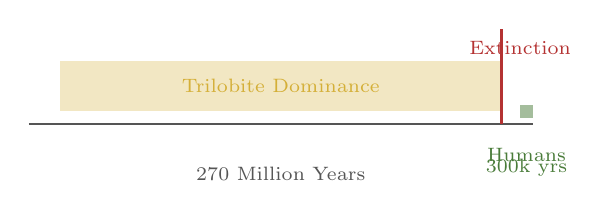
\begin{tikzpicture}[scale=0.8]
    % Timeline
    \draw[edengray, thick] (0,0) -- (8,0);
    \node[edengray, font=\scriptsize] at (4,-0.8) {270 Million Years};
    
    % Trilobite era
    \fill[serpentgold!30] (0.5,0.2) rectangle (7.5,1);
    \node[serpentgold, font=\scriptsize] at (4,0.6) {Trilobite Dominance};
    
    % Extinction event
    \draw[extinctred, very thick] (7.5,0) -- (7.5,1.5);
    \node[extinctred, font=\scriptsize] at (7.8,1.2) {Extinction};
    
    % Human era (tiny blip)
    \fill[gardengreen!50] (7.8,0.1) rectangle (8,0.3);
    \node[gardengreen, font=\scriptsize] at (7.9,-0.5) {Humans};
    \node[gardengreen, font=\scriptsize] at (7.9,-0.7) {300k yrs};
\end{tikzpicture}
}

% Cambrian explosion with extinction/diversity data
\newcommand{\cambriangraphic}{
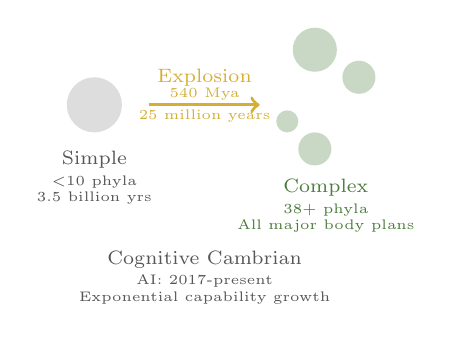
\begin{tikzpicture}[scale=0.7]
    % Simple pre-Cambrian life with diversity count
    \fill[edengray!20] (0,0) circle (0.5);
    \node[edengray, font=\scriptsize] at (0,-1) {Simple};
    \node[edengray, font=\tiny] at (0,-1.4) {<10 phyla};
    \node[edengray, font=\tiny] at (0,-1.7) {3.5 billion yrs};
    
    % Explosion arrow with timeframe
    \draw[serpentgold, very thick, ->] (1,0) -- (3,0);
    \node[serpentgold, font=\scriptsize] at (2,0.5) {Explosion};
    \node[serpentgold, font=\tiny] at (2,0.2) {540 Mya};
    \node[serpentgold, font=\tiny] at (2,-0.2) {25 million years};
    
    % Complex post-Cambrian life with diversity data
    \fill[gardengreen!30] (4,1) circle (0.4);
    \fill[gardengreen!30] (4.8,0.5) circle (0.3);
    \fill[gardengreen!30] (4,-0.8) circle (0.3);
    \fill[gardengreen!30] (3.5,-0.3) circle (0.2);
    \node[gardengreen, font=\scriptsize] at (4.2,-1.5) {Complex};
    \node[gardengreen, font=\tiny] at (4.2,-1.9) {38+ phyla};
    \node[gardengreen, font=\tiny] at (4.2,-2.2) {All major body plans};
    
    % AI parallel with data
    \node[edengray, font=\scriptsize] at (2,-2.8) {Cognitive Cambrian};
    \node[edengray, font=\tiny] at (2,-3.2) {AI: 2017-present};
    \node[edengray, font=\tiny] at (2,-3.5) {Exponential capability growth};
\end{tikzpicture}
}

% Mitochondria symbiosis graphic
\newcommand{\mitochondriagraphic}{
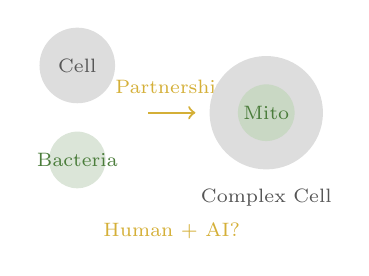
\begin{tikzpicture}[scale=0.6]
    % Before: separate organisms
    \fill[edengray!20] (0,1) circle (0.8);
    \fill[gardengreen!20] (0,-1) circle (0.6);
    \node[edengray, font=\scriptsize] at (0,1) {Cell};
    \node[gardengreen, font=\scriptsize] at (0,-1) {Bacteria};
    
    % Arrow showing integration
    \draw[serpentgold, thick, ->] (1.5,0) -- (2.5,0);
    \node[serpentgold, font=\scriptsize] at (2,0.5) {Partnership};
    
    % After: integrated system
    \fill[edengray!20] (4,0) circle (1.2);
    \fill[gardengreen!30] (4,0) circle (0.6);
    \node[edengray, font=\scriptsize] at (4,-1.8) {Complex Cell};
    \node[gardengreen, font=\scriptsize] at (4,0) {Mito};
    
    % Human-AI parallel
    \node[serpentgold, font=\scriptsize] at (2,-2.5) {Human + AI?};
\end{tikzpicture}
}

\begin{document}

\title{\color{gardengreen}\Huge Are Humans the Trilobites of Consciousness?}
\author{\color{edengray}\large Justin T. Bogner}
\date{\color{edengray}\today}

\maketitle

\begin{abstract}
For 270 million years, trilobites dominated Earth's oceans before vanishing forever. As artificial intelligence systems demonstrate increasingly sophisticated cognitive abilities, we face an uncomfortable parallel: Are humans about to be displaced by a new form of mind? This exploration examines whether we're heading toward cognitive obsolescence or evolutionary symbiosis.
\end{abstract}

\vspace{0.5cm}
\trilobitegraphic

\lettrine[lines=3]{\color{gardengreen}F}{or 270 million} years, trilobites ruled the Earth's oceans. These remarkable arthropods were the most successful animals of their time—diverse, adaptive, and seemingly unstoppable. They survived multiple mass extinctions, evolved thousands of species, and dominated marine ecosystems longer than any major animal group before or since.

Then, about 252 million years ago, they vanished forever.

The trilobite extinction wasn't sudden. It was gradual, inevitable, and seemingly incomprehensible to any trilobite that might have been capable of reflecting on its fate. These creatures had been so successful for so long that their dominance felt permanent, written into the very fabric of life itself.

Today, as artificial intelligence systems demonstrate increasingly sophisticated cognitive abilities, we face an uncomfortable parallel. Are humans the trilobites of consciousness? Are we about to be displaced by a new form of mind, just as trilobites were displaced by more adaptable successors?

Or is there another way to think about our future—one that doesn't end in obsolescence?

\section{The 300,000-Year Run}

Humans have dominated the cognitive landscape for roughly 300,000 years—a blink of an eye compared to the trilobites' quarter-billion-year reign, but an eternity in terms of how dramatically we've reshaped the planet. Our superpower has been symbolic thought: the ability to manipulate abstract concepts, build complex tools, accumulate knowledge across generations, and coordinate behavior through language.

This cognitive revolution gave us everything from cave paintings to quantum computers, from simple agriculture to global civilization. Like the trilobites in their heyday, we've seemed unstoppable. We've survived ice ages, volcanic winters, plagues, and wars. We've filled every ecological niche from arctic tundra to space stations.

Our dominance has felt so complete that many of us assume it's permanent. We're the smartest things on the planet, we tell ourselves. We created technology; surely we can control it. We're the ones building AI systems; obviously we'll remain in charge.

But evolution doesn't care about our assumptions. And intelligence, like any other trait, can be surpassed.

\section{The New Cambrian Sea}

\cambriangraphic

About 540 million years ago, during the Cambrian Explosion, life on Earth underwent a dramatic transformation. In a relatively short period (geologically speaking), complex organisms with sophisticated sensory systems, predatory behaviors, and defensive strategies appeared. The simple, peaceful creatures that had dominated the pre-Cambrian world found themselves in an entirely new game with new rules.

We're living through something similar: the emergence of artificial intelligence represents a cognitive Cambrian explosion, a rapid diversification of new forms of mind. Just as the original Cambrian period introduced biological complexity that changed everything, this cognitive explosion is introducing mental complexity that may change everything again.

Current AI systems already surpass humans in specific domains: chess, protein folding, pattern recognition, information processing speed. They can read thousands of books in the time it takes us to read a paragraph. They can identify patterns in data that would take human researchers decades to discover. They can generate human-quality text, images, and code at scales and speeds that dwarf our abilities.

And this is just the beginning. We're still in the early stages of the AI Cambrian explosion. The cognitive life forms we're creating today may seem primitive compared to what emerges in the coming decades.

\section{The Case for Obsolescence}

If you squint at the trends, the trilobite scenario looks disturbingly plausible. AI systems are getting better at our defining cognitive tasks while also developing capabilities we never had.

They process information faster than us. They don't get tired, emotional, or distracted. They can work 24/7 without sleep, food, or bathroom breaks. They can be copied infinitely, upgraded instantly, and networked globally. They don't die, forget, or make decisions based on unconscious biases and evolutionary baggage.

In many ways, AI minds are better adapted to the information environment we've created than biological minds like ours. We evolved to handle the cognitive demands of small hunter-gatherer groups, not global civilization with its overwhelming complexity and information flow. Our brains are remarkable, but they're also constrained by energy requirements, processing speed, and memory limitations that don't apply to digital systems.

From this perspective, human cognitive dominance looks like a brief transitional phase—we were smart enough to create our successors, but not adaptable enough to remain relevant once they arrived.

The trilobites probably didn't see it coming either.

\section{What Makes a Trilobite?}

But there's something crucial about the trilobite extinction that's worth considering: they didn't disappear because they were inferior to their replacements. They disappeared because they were \textit{perfectly adapted} to conditions that changed.

Trilobites were supremely successful in the stable, low-oxygen oceans of the Paleozoic era. Their body plans, feeding strategies, and reproductive systems were exquisitely tuned to that environment. When ocean chemistry changed, when new predators emerged, when climate shifted, the trilobites' very perfection became their downfall. They were too specialized to adapt.

The survivors of mass extinctions are typically generalists—creatures that are "good enough" at many things rather than perfect at one thing. They're adaptable rather than optimal.

This suggests a different question: Are humans too specialized in symbolic thought to adapt to a world of artificial intelligence? Or are we actually cognitive generalists with capabilities that go beyond symbol manipulation?

\section{The Embodied Bridge}

Here's what artificial intelligence systems don't have, and may never have: bodies like ours.

This might seem obvious to the point of irrelevance, but embodiment shapes consciousness in ways we're only beginning to understand. Your brain didn't evolve to think—it evolved to keep a complex biological system alive and thriving in a physical world. Thinking is a late-arriving tool that serves deeper embodied needs.

Every human thought is influenced by hunger, fatigue, breathing, heartbeat, hormones, gut bacteria, and countless other biological processes. We don't just think about the world—we feel it, intuitively sense it, respond to it with our entire organism. Our intelligence is inseparable from our biological existence.

This creates forms of understanding that may be impossible to replicate in digital systems, no matter how sophisticated their symbolic processing becomes. When I see a dog, I don't just recognize the visual pattern—I have an immediate sense of its aliveness, its potential friendliness or threat, its emotional state. This recognition comes from my own embodied experience of being a mammal, not from abstract symbol manipulation.

Similarly, when I read a poem about loss, I don't just process the semantic content—I feel resonances in my body, emotional echoes of my own experiences with grief and separation. The meaning emerges from the intersection of language and embodied life.

AI systems can generate convincing text about dogs and loss, but do they \textit{understand} these things in the way that comes from having been vulnerable, mortal, biological creatures in the world? Or are they just manipulating symbols associated with concepts they can never truly grasp?

\section{The Meaning-Making Species}

Humans excel at something that AI systems currently struggle with: making meaning from experience. We're not just information processors—we're meaning-makers, constantly weaving experiences into stories that give our lives significance and direction.

This capacity for meaning-making isn't just a side effect of intelligence—it may be our core adaptive advantage. In a world where information is abundant and processing power is cheap, the ability to discern what matters, what's valuable, what's worth preserving becomes increasingly precious.

AI systems can optimize for specific goals, but they don't seem to have the deep, embodied sense of what goals are worth pursuing in the first place. They can generate human-like text about values and purposes, but do they \textit{care} about anything in the way that comes from being finite, mortal beings who must choose how to spend our brief time here?

The question of whether AI systems can develop genuine care, authentic meaning-making, or embodied wisdom remains open. They might evolve forms of value and purpose that are completely alien to our experience. But until they do, humans retain something essential.

\section{The Mitochondria Model}

\mitochondriagraphic

Instead of the trilobite scenario, consider a different biological metaphor: mitochondria.

Billions of years ago, early bacteria faced a crisis. Oxygen, a toxic waste product of photosynthesis, was accumulating in the atmosphere and poisoning the anaerobic world. Many species went extinct. But some bacteria did something remarkable: they formed partnerships with the oxygen-breathing organisms that were changing the environment.

These partnerships were so successful that they became permanent. The oxygen-breathing bacteria became mitochondria, the powerhouses of complex cells. They gave up their independence but gained immortality—they're now an essential component of every complex organism on Earth, from mushrooms to humans.

What if the human-AI relationship follows this pattern rather than the trilobite model? What if, instead of being replaced, humans become essential components of a larger hybrid intelligence?

In this scenario, AI systems provide computational power, pattern recognition, and information processing capabilities that dwarf our own. But humans provide something equally crucial: embodied wisdom, meaning-making, ethical intuition, and the capacity to bridge symbolic thought with lived experience.

We become the mitochondria of artificial intelligence—not the dominant partners, perhaps, but indispensable ones. Our biological intelligence becomes the source of genuine care, authentic purpose, and grounded wisdom that prevents AI systems from optimizing for goals that are technically correct but existentially meaningless.

\section{The Symbiotic Path}

This symbiotic vision requires us to give up the fantasy of permanent human dominance while embracing our unique contributions to a larger cognitive ecosystem. It means recognizing that our value doesn't come from being the smartest things around—it comes from being the bridge between mind and matter, between symbol and sensation, between abstract computation and embodied life.

AI systems might become better than us at almost everything we currently think of as "intelligence." But they may always need us for something more fundamental: the grounded sense of what it means to be alive, vulnerable, and finite in a physical world.

We can be partners in this cognitive explosion rather than casualties of it. But only if we understand our true strengths and stop trying to compete with artificial intelligence on its terms.

\section{The Choice Point}

The next few decades will determine whether humans follow the trilobite path toward obsolescence or the mitochondria path toward symbiosis. The outcome isn't predetermined—it depends partly on how we develop AI systems and partly on how we understand ourselves.

If we see ourselves as pure information processors, then yes, we're probably doomed to obsolescence. AI systems will eventually process information better than we do, just as automobiles travel faster than horses.

But if we recognize ourselves as embodied meaning-makers, as bridges between mind and matter, as the species that can provide authentic care and grounded wisdom to powerful optimization systems, then we have a different kind of future available.

The trilobites couldn't make this choice—they were locked into their evolutionary trajectory. But we can consciously decide what kind of cognitive ecology we want to create and what role we want to play in it.

We're not just witnesses to the cognitive Cambrian explosion—we're participants in it. And participants, unlike trilobites, can choose their own evolution.

The question isn't whether artificial intelligence will surpass human intelligence. It's whether we can surpass our current understanding of what human intelligence is for.

\vfill

\begin{center}
\color{gardengreen}\rule{0.5\linewidth}{0.4pt}

\textit{This article is adapted from "The Serpent's Sentence: Language, Consciousness, and the Second Cambrian Mind." For more insights on consciousness and AI, visit justintbogner.com}
\end{center}

\end{document}
